\documentclass[article]{article}
\usepackage{amsmath,amsthm,bm,mathrsfs,amssymb, float}
\usepackage[a4paper, total={6in, 9in}]{geometry}
\usepackage[colorlinks]{hyperref}
\usepackage{graphicx}
\usepackage{subcaption}

\title{Numerical Algorithms – Assignment 3}
\author{Kahaan Shah \& Santripta Sharma}
\date{\today}

\setlength{\parindent}{0px}

\begin{document}

\maketitle

\section{Introduction}
For this assignment we have implemented facial recognition using the Eigenfaces method on a dataset of 400 face images. The goal of the assignment is to take an input of pictures of people and be able to  create a model such that, when given a new image of the same person, it can match them to their other images.

\section{Data}
We used a data set of 400 faces called the \href{https://paperswithcode.com/dataset/olivetti-face}{Olivetti Face} dataset. The dataset consists of 400 $64 \times 64$ images of faces. There are 40 individual people, with 10 images per person in the dataset. The images are all black and white and centred on the nose, but sometimes have a slight side profile of the person rather than a front face photo each time. We had a train-test split of $70:30$. sampling 7 images for each person at random.

\section{Eigenfaces}

\subsection{Input Matrix}

The Eigenfaces technique is largely based on PCA. To construct our input matrix we flatten each image from $64 \times 64$ to $4096 \times 1$. These vectors then form the columns of our input matrix constructing a train input matrix of $4096 \times 280$. \bigskip

We also mean centre the images, subtracting the mean pixel value of every image from the pixels in the image. Let the (flattened) mean face of our training set be represented by $\mathbf{\Psi} \in \mathbb{R}^{4096}$, which we will use later while embedding faces.

\subsection{Singular Value Decomposition}
To conduct PCA on this matrix we need to find the eigenvectors of its covariance matrix. We note that our input matrix $\mathbf{A}$ can be written as $\mathbf{A} = \mathbf{U \Sigma V}^\top$. We then have the covariance matrix $ \frac{\mathbf{A} \mathbf{A}/n ^\top}{n} = \frac{\mathbf{U \Sigma V}^\top (\mathbf{U \Sigma V}^\top) ^\top}{n} = \frac{\mathbf{U \Sigma \Sigma ^\top U^\top}}{n}$. Since this is a positive symmetric matrix, we know that the eigenvalues are given by $ \frac{\mathbf{\Sigma \Sigma}^\top}{n}  = \frac{\mathbf{\Sigma}^2}{n}$ and the eigenvectors are the columns of $\mathbf{U}$. We then unstack the eigenvectors to retrieve the eigenfaces.

\begin{figure}[H]
    \centering
    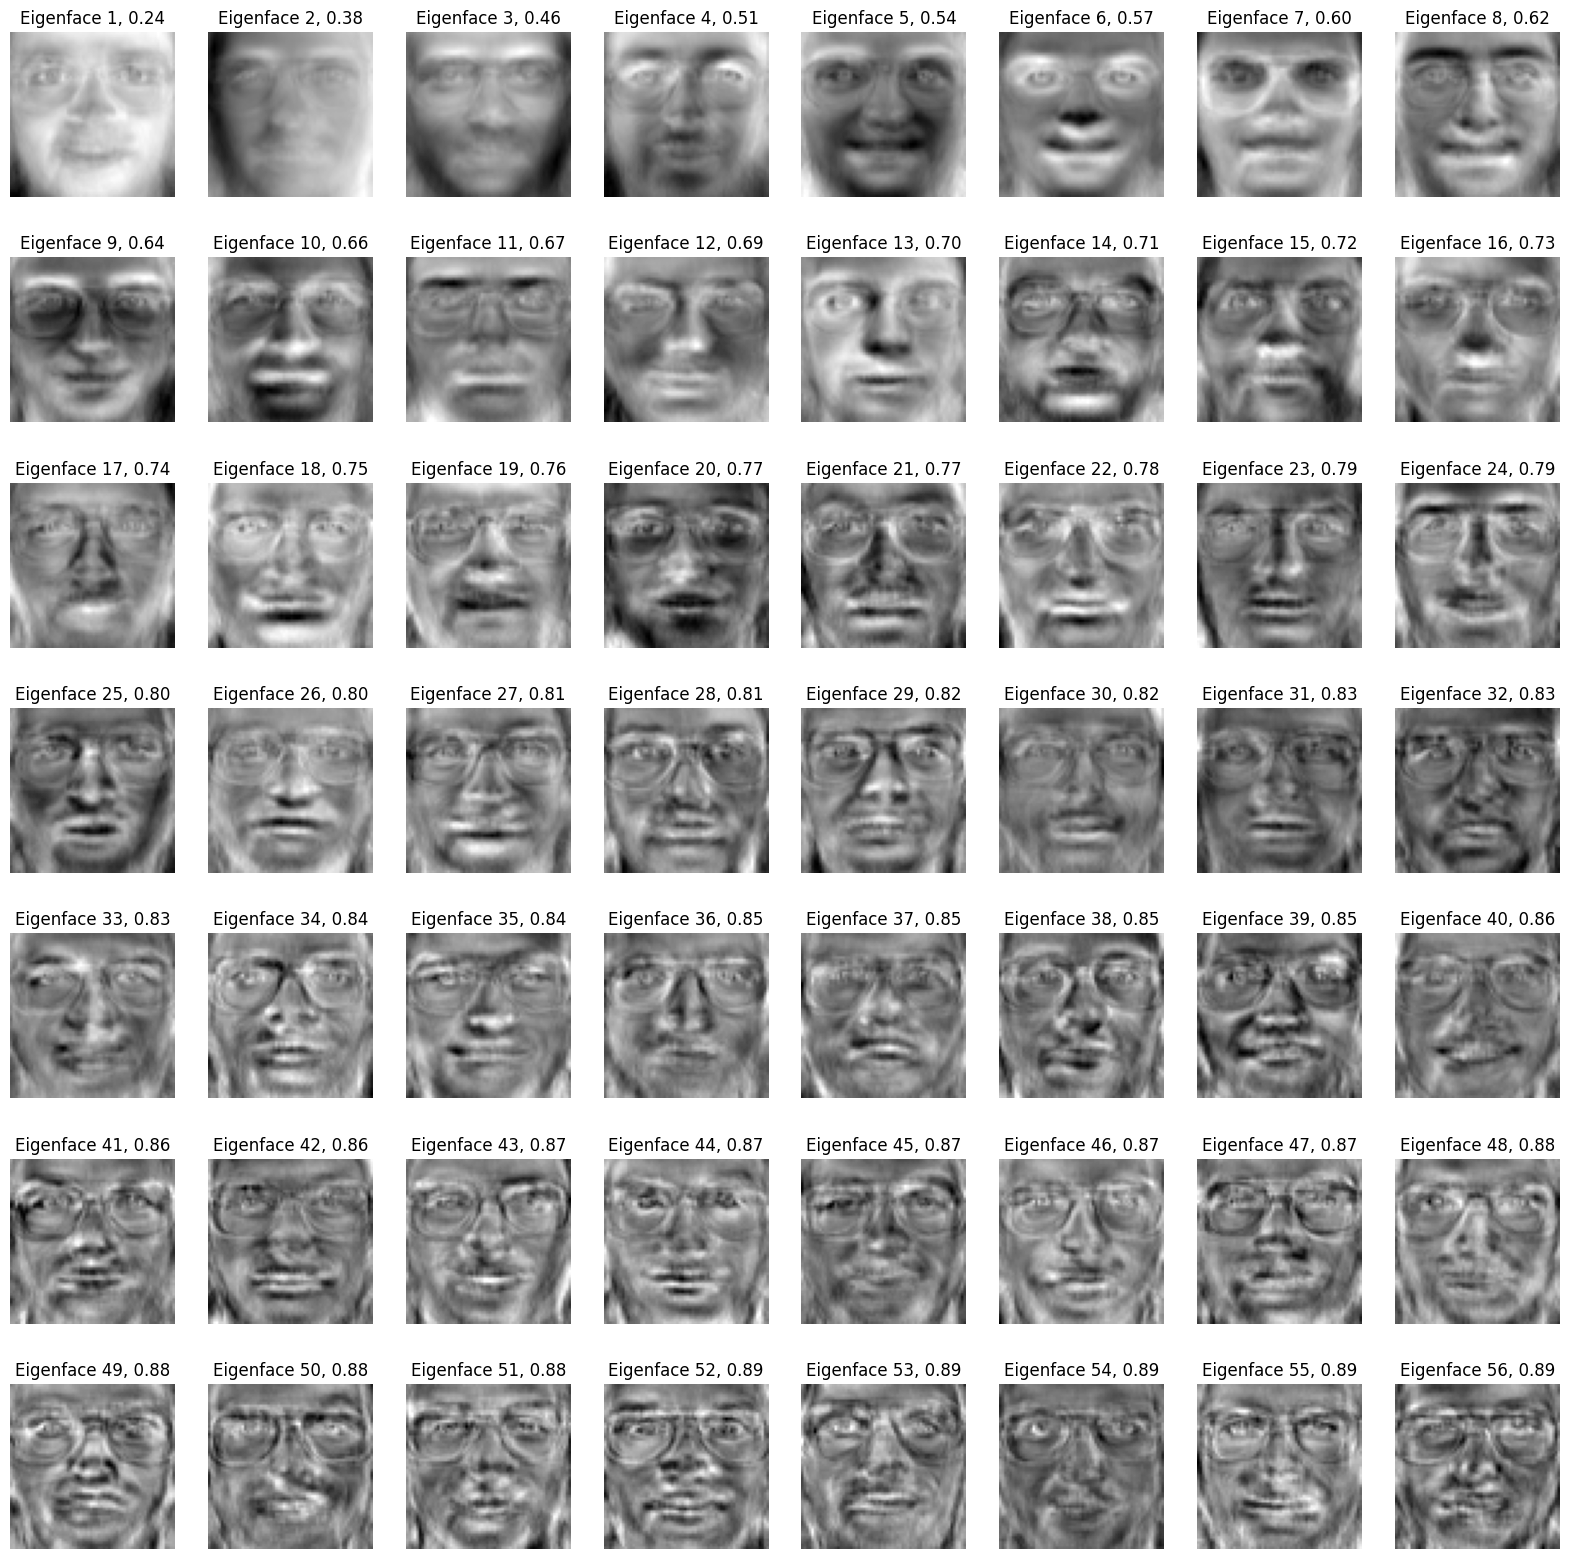
\includegraphics[width=1\linewidth]{eigenfaces-variance.png}
    \caption{Eigenfaces, along with the cumulative \% of the sum of eigenvalues up to that eigenface}
    \label{fig:eigenfaces}
\end{figure}

With our given train/test split (fixed seed), we require only 104 eigenfaces (compared to the total 280 in the training set), to represent $>95\%$ of the variance in the training set faces. Let the "principal" eigenfaces then be $\mathbf{E = [E_1, E_2, \dots, E_{104}]} \in \mathbb{R}^{4096\times 104}$

%Add plots here with notes

\subsection{Embedding a Face into the EigenFaceSpace}

Given an image $\mathbf{I_0} \in \mathbb{R}^{64\times 64}$, we first flatten it, retrieving $\mathbf{I} \in \mathbb{R}^{4096}$ and then center it to the mean of our training set, $\bf I' = I - \Psi$. Finally, in order to embed it into our eigenbasis, we project it onto each basis element, giving us our final embedding, $\mathbf{E_I = (I'\cdot E_1, I'\cdot E_2, I'\cdot E_3, \dots, I'\cdot E_{104})}$.

\section{Reconstruction}

We can now try seeing how well this relatively small basis is able to reconstruct the faces, both in our test, and train sets. The reconstruction procedure is outlined below:

\begin{enumerate}
    \item First, take the flattened input image $\bf I$ and embed it into the space as $\mathbf{E_I} \in \mathbb{R}^{104}$
    \item Recover the flattened reconstructed image $\bf R$ by taking the linear combination of the eigenvectors weighted by $\mathbf{E_I}$, $\mathbf{R} = \mathbf{E_I}\mathbf{E^t}$
    \item Unflatten the image to get $\mathbf{R_0} \in \mathbb{R}^{64\times 64}$.
\end{enumerate}

To gauge the accuracy of this method, we use two pixel-wise losses, the mean square error, and absrel, given by $\text{MSE}(x, \hat{x}) = \langle(x - \hat{x})^2\rangle, \text{AbsRel}(x, \hat{x}) = \langle|x - \hat{x}|/x\rangle$.\bigskip

We use a valid mask in the absrel case to exclude any pixels with value $0$ from the mean.\bigskip

We also vary the number of principal eigenfaces we use, instead of sticking to $104$. This is parametrised as $k$. Our metrics on the train and test set can be seen below:

\begin{center}
    \begin{tabular}{|c|c|c|c|c|}
        \hline \textbf{Set} & \textbf{MSE ($k = 104$)} & \textbf{MSE ($k = 250$)} & \textbf{AbsRel ($k = 104$)} & \textbf{AbsRel ($k = 250$)} \\
        \hline Train & 9.68e-4 & 4.43e-5 & 5.38e-2 & 9.96e-3 \\
        \hline Test & 2.53e-3 & 1.79e-3 & 8.57e-2 & 7.13e-2\\
        \hline
    \end{tabular}    
\end{center}

Here, we can see that while increasing the size of the basis to almost contain all the eigenfaces leads to a steep decline in the metrics for the training dataset ($> 1/2$ an order, which is to be expected), the gains in the test dataset seem to come much slower, which seems to point to the limited ability of this approach, at least with this size/type of dataset, to generalise beyond its training set.\bigskip

\begin{figure}[h]
    \centering
    \begin{subfigure}{.5\textwidth}
      \centering
      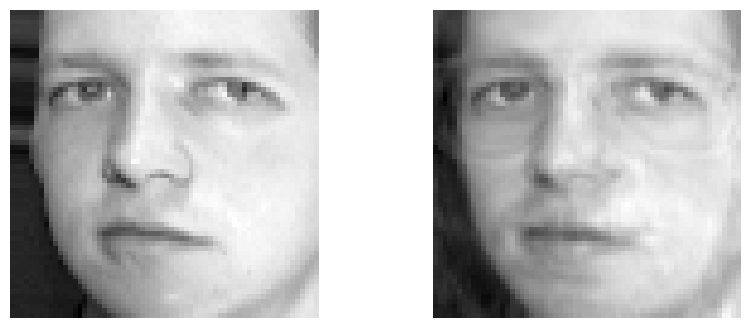
\includegraphics[width=.8\linewidth]{eigenfaces-104-recon.png}
      \caption{$k = 104$, original on the left}
      \label{fig:sfig1}
    \end{subfigure}%
    \begin{subfigure}{.5\textwidth}
      \centering
      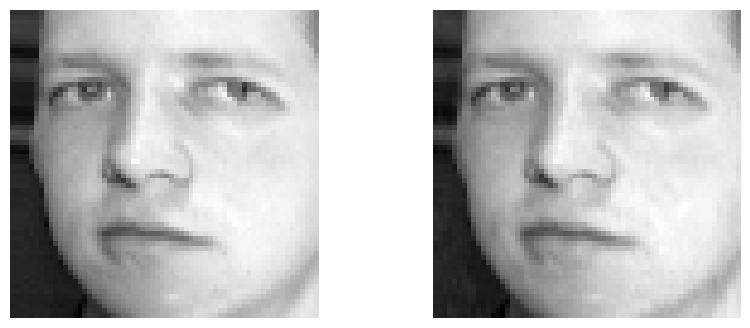
\includegraphics[width=.8\linewidth]{eigenfaces-250-recon.png}
      \caption{$k = 250$, original on the left}
      \label{fig:sfig2}
    \end{subfigure}
    \caption{\centering Reconstructing a member of the training set with varying values of $k$. We can see how (a) seems to have obvious artifacts, for instance, the "phantom glasses" appearing over the reconstructed face, whereas such artifacts are less apparent in (b)}
\end{figure}

\section{Facial Recognition}
The eigenfaces approach can also be used to detect facial similarity between a "face database" and an incoming face picture, which can be applied in various face-based authentication systems. We investigate the suitability of such an approach by setting up our face database, by simply embedding all of our training set images into the eigenspace, giving us $\mathbf{D}\in \mathbb{R}^{104\times 280}$ (280 being the number of training set images).\bigskip

Now, given the embedding of a "query image", $\bf E_I$, we can simply take the dot products (cosine similarity) between $\bf E_I$ and each column of $\bf D$, which can be represented as a vector $\bf S^t = E_I^t D$.\bigskip

Taking the index corresponding to the maximum entry in $\bf S$ gives us the index of the training set image that best matches our query image.\bigskip

To evaluate the success of this method, we use our training set as our face database, and images from our test or training sets as the queries. We count a success when the closest match to our query image is one of the $7$ training images from the same individual. Then we have the accuracies, for varying values of $k$:

\begin{center}
    \begin{tabular}{|c|c|c|}
        \hline $\bf k$ & Accuracy (train) & Accuracy (test)  \\
        \hline 10 & 50.36\% & 44.17\% \\
        \hline 50 & 84.64\% & 63.34\% \\
        \hline 104 & 91.43\% & 67.5\% \\
        \hline 150 & 93.21\% & 67.5\% \\
        \hline 250 & 95\% & 69.17\%\\
        \hline
    \end{tabular}
\end{center}

We see that while the train accuracy continues growing, the test accuracy plateaus near $70\%$, which means that in the case of authentication, $30\%$ of authentications were misauthentications, providing access to someone who should not have access, in the worst case. We've displayed a failure case below:

\begin{figure}[H]
    \centering
    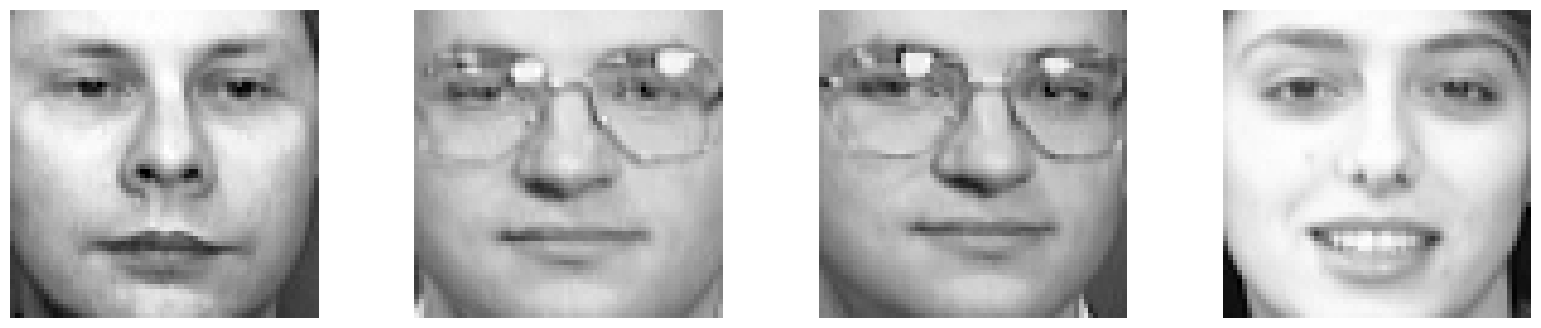
\includegraphics[width=1\linewidth]{eigenfaces-recognition-failure.png}
    \caption{\centering Recognition failure, the leftmost face is the query, and the next $3$ faces are the $3$ closest faces in descending order}
    \label{fig:eigenfaces-failure}
\end{figure}

\end{document}